\documentclass{beamer}
%\usepackage{split}

\usepackage{amsmath}
\usepackage{amsfonts}
\usepackage{braket}
\usepackage{subcaption}
\usepackage{tikz}
\usepackage{xcolor}
\usetikzlibrary{positioning,shapes,arrows.meta}
%\usetikzlibrary{positioning,fit,backgrounds}
\usepackage{quantikz}
\usepackage[linesnumbered]{algorithm2e}
\usepackage{hyperref}
%\usepackage{hyperref,xcolor}
%\usepackage[ocgcolorlinks]{ocgx2}
\usepackage{cleveref}
\usepackage[backend=biber,style=authoryear,sorting=ynt]{biblatex}
\addbibresource{./sample.bib}


\newcommand*{\QACze}{ \mathbf{QAC}_{0} }
\newcommand*{\QNCzef}{ \mathbf{QNC}_{0,f} }
\newcommand*{\QNCze}{ \mathbf{QNC}_{0} }
\newcommand*{\QNCon}{ \mathbf{QNC}_{1} }
\newcommand*{\NCon}{ \mathbf{NC}_{1} }
\newcommand*{\noiseQNCon}{ noisy-$\QNCon$ }
\newcommand*{\QNC}{ \mathbf{QNC} }
\newcommand*{\QNCG}{ \mathbf{QNC_G} }
\newcommand*{\NC}{\mathbf{NC}}
\newcommand*{\QNCiG}{\mathbf{QNC_{G,i}}}


\begin{document} 

\newcommand*{\Tr}{\textbf{Tr }}


\begin{frame}
  \title{Does $\QNCon =$ \noiseQNCon ? }
    \author{David Ponarovsky}
    \date{\today}
    \titlepage
\end{frame}


\begin{frame}

\frametitle{Introduction}
\begin{block}{Today:}
\begin{itemize}
  \item Noisy Circuits.
  \item  Definitions and Motivation.
  \item  Pippenger Construction. (Classical, Fault Tolerance with constant overhead at depth ).
  \item `Franch-line' works, modern fault tolerance methods and gadgets. ('log n' overhead at depth).  
  \item Next week, directions and hints that might show separation. ($\neq$).
\end{itemize}
\end{block}
\begin{block}{TAKEAWAYS:}
\begin{itemize}
  \item More about codes.
  \item  First view to fault tolerance.  
\end{itemize}
\end{block}
\end{frame}



\begin{frame}
  \frametitle{Nosiy Circuit.}

\begin{quantikz}[row sep=0.3cm, column sep=0.7cm]
\lstick{$q_1$} & \gate[wires=8]{U_0} & \gate{\mathcal{N}} & \gate[wires=8]{U_1}   & \gate{\mathcal{N}} & \gate[wires=8]{U_2} & \gate{\mathcal{N}}& \qw \\
\lstick{$q_2$} &                      & \gate{\mathcal{N}} &                      & \gate{\mathcal{N}} &                     & \gate{\mathcal{N}} & \qw \\
\lstick{$q_3$} &                      & \gate{\mathcal{N}} &                      & \gate{\mathcal{N}} &                     & \gate{\mathcal{N}} & \qw \\
\lstick{$q_4$} &                      & \gate{\mathcal{N}} &                      & \gate{\mathcal{N}} &                     & \gate{\mathcal{N}} & \qw \\
\lstick{$q_5$} &                      & \gate{\mathcal{N}} &                      & \gate{\mathcal{N}} &                     & \gate{\mathcal{N}} & \qw \\
\lstick{$q_6$} &                      & \gate{\mathcal{N}} &                      & \gate{\mathcal{N}} &                     & \gate{\mathcal{N}} & \qw \\
\lstick{$q_7$} &                      & \gate{\mathcal{N}} &                      & \gate{\mathcal{N}} &                     & \gate{\mathcal{N}} & \qw \\
\lstick{$q_8$} &                      & \gate{\mathcal{N}} &                      & \gate{\mathcal{N}} &                     & \gate{\mathcal{N}} & \qw
\end{quantikz}
\end{frame}

\begin{frame}{Nosiy Circuit.}
  \begin{definition}{ $p$- Depolarizing Channel. } 
    The qubit depolarizing channel with parameter $ p \in [0,1] $ is the quantum channel $ \mathcal{D}_p $ defined by:
\begin{equation*}
  \begin{split}
\mathcal{D}_p(\rho) = (1 - p) \rho + p \cdot \frac{I}{2}
  \end{split}
\end{equation*}

where $ \rho $ is a single-qubit density matrix and $ I $ is the identity matrix.

  \end{definition}
  \begin{definition}{$p$-Noisy Circuit.}
    Given a circuit $C$ (regardless of the model), its $p$-noisy version $\tilde{C}$ is the circuit obtained by alternately taking layers from $C$ and then passing each (qu)bit through a $p$-Depolarizing channel.
  \end{definition}
\end{frame}


\begin{frame}
  \frametitle{Threshold Theorem.} 
  \begin{theorem}[Threshold Theorem. Informal.]
There is a universal $p_{th} \in (0,1)$ such that for any $p < p_{th}$, any circuit in BQP can be simulated by a $p$-noisy BQP circuit. The simulating circuit has a depth that is at most $\text{poly} \log n$ times the original depth.
  \end{theorem}

\begin{figure}[h]
    \centering
    \includegraphics[width=\textwidth]{threshold.png}
    \caption{Caption for the image}
    \label{fig:your-label}
\end{figure}
\end{frame}

\begin{frame}
  \frametitle{Threshold Theorem.} 

\end{frame}


\begin{frame}{Definition}
%  \begin{block}{Definition}
\begin{definition}[$\NC$ - Nick's Class]
$\NC_i$ is the class of decision problems solvable by a uniform family of Boolean circuits, with polynomial size, depth $O(\log^i(n))$, and fan-in $2$. 
\end{definition}

\begin{definition}[$\QNC$]
  The class of decision problems solvable by polylogarithmic-depth, and finate fan out/in quantum circuits with bounded probability of error. Similarly to $\NC_i$, $\QNC_i$ is the class where the decisdes the circuits have $\log^i (n)$ depth.  
\end{definition}

\begin{definition}[$\QNCG$]
  For a fixing finate fan in/out gateset $G$, the class with deciding circuits composed only for gates in $G$ and at depath at most polylogaritmic. And in similar to $\QNC_{i}$, $\QNCiG$ is the restirction to circuits with depath at most $\log^{i}(n)$.  
\end{definition}
 % \end{block}
\end{frame}

\begin{frame}
  \frametitle{Pippenger's Construction.} 
  
  \begin{theorem}[Threshold Theorem - Pippenger. Informal.]
    There is fault tolerance construction with a constant depth overhead.
  \end{theorem}
Encode each bit with the repetition code $0 \mapsto 0^{m}$, $1 \mapsto 1^{m}$. Now observe that any logical operation, without decoding, can be made in $O(1)$ depth.

For example, OR($\bar{x}, \bar{y}$) can be computed by applying in parallel OR($x_{i}, y_{i}$) for each $i$.

\end{frame}


\begin{frame}
  \frametitle{The 'Decoding' trick.} 

Instead of completely decoding, we would apply only a single step of partial decoding. We assume that in each code block the bits are partitioned into random disjoint triples, and we will apply a local correction to each of the triples by majority.



\begin{block}{Claim}
There are constants $\alpha, \eta \in (0,1)$ such that for any bit string $x$ at a distance $\le \alpha n$ from the code (Repetition Code), one cycle of local correction on $x$ yields $x^\prime$ such that:
  \begin{equation*}
    \begin{split}
      d(x^{\prime}, C) \le d(x, C)
    \end{split}
  \end{equation*}
\end{block}
\end{frame}


\begin{frame}
  \frametitle{The 'Decoding' trick.} 
  
  Suppose that a bit obserb a bit flip with probability $p$. So in expectation we expect that entire bolck at length $n$ will absorb $pn$ flips.  
  \begin{equation*}
    \begin{split}
      \eta \left( \beta + p  \right) n &\le \beta n \\ 
      \beta \ge \frac{p}{ 1 - \eta}
    \end{split}
  \end{equation*}


\end{frame}

\begin{frame}{The Decoding Algorithm.}
  First noitce that the repetition code could be defined as Tanner code, for any $\Delta$-regular graph $G$ and local code $C_{0}$ which is the repetition over $\Delta$ bits.   


  In particular $G$ could be a bipartite expander graph. Denote the right and the left vertices subsets by $V^{-}$ and $V^{+}$.
  \begin{block}{Decoding:}
    For $\Omega\left( \log n \right)$ iterations, do: 
  \begin{enumerate}
    \item In every even iteration, all the vertices in $V^{+}$ 'correct' their local view based on the majority.
    \item In every odd iteration, all the vertices in $V^{-}$ 'correct' their local view based on the majority.
  \end{enumerate}
For having a constant depth error reduction procedure, it's enough to run the decoding above for two iterations.
\end{block}

\end{frame}


\begin{frame}{The Decoding Algorithm.}

  
  \begin{figure}[h]
    \begin{subfigure}[h]{0.4\textwidth}

    \label{alg:three}
      \begin{algorithm}[H]
    \KwData{ $x \in \mathbb{F}_{2}^{n}$ }
    \For { $ v \in V^{+}$} {
      $x^{\prime}_{v} \leftarrow \arg\min {\left\{  y \in C_{0} : |y + x|_{v} |  \right\} } $\\
    }
    \For { $ v \in V^{-}$} {
      $x^{\prime}_{v} \leftarrow \arg\min {\left\{  y \in C_{0} : |y + x|_{v} |  \right\} } $\\
    }
    \Return  $x $

  \end{algorithm}
    \end{subfigure}
    \begin{subfigure}[h]{0.1\textwidth}
      \
    \end{subfigure}
    \begin{subfigure}[h]{0.45\textwidth} 

    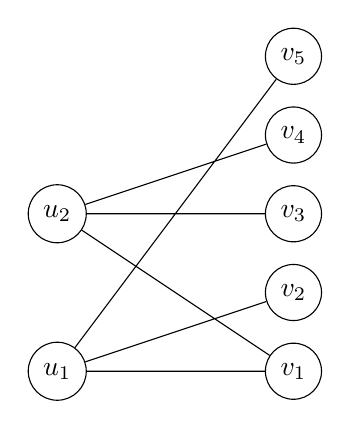
\begin{tikzpicture}%[scale=2.5]
\tikzstyle{every node}=[draw,shape=circle];

\draw node (v0) at (0,1) {$u_1$};
\draw node (v6) at (0,3) {$u_2$};
\draw node foreach \x in {1,2,3,4,5} (v\x) at (3,\x) {$v_\x$};

\draw (v0) -- (v1)
(v0) -- (v2)
(v0) -- (v5)
(v6) -- (v3)
(v6) -- (v4)
(v6) -- (v1);
\end{tikzpicture}
    \label{fig:location}
    \end{subfigure} 
  \end{figure}

\end{frame}
\begin{frame}{The Decoding Algorithm.}

  \begin{lemma}
    \label{lemma:reduce}
There exists $\beta \in (0,1)$ such that if the error is at weight less than $\beta n$, then a single correction round reduces the error by at least a $\frac{1}{2}$ fraction.
  \end{lemma}

\end{frame}
\begin{frame}{The Decoding Algorithm.}
  \begin{block}{Proof.}
  Denote by $S^{(0)} \subset V^{+}$ and  $T^{(0)} \subset V^{-}$ the subsets of left and right vertices adjacent to the error. And denote by $T^{(1)} \subset T^{(0)}$ the right vertices such any of them is connect by at least $\frac{1}{2}\Delta$ edges to vertices at $S^{(0)}$. \\~\

  Note that that any vertex in $V^{-}/T^{(1)}$ has on his local view less than $\frac{1}{2}\Delta$ faulty bits, So it corrects into his right local view in the first right correction round. \\~\

  Therefore after the right correction round the error is set only on $T^{(1)}$'s neighbourhood, namely at size at most $\Delta|T^{(1)}|$. We will show:
  \begin{equation*}
    \begin{split}
  \Delta|T^{(1)}| \le \text{constant} \cdot |e|
    \end{split}
  \end{equation*}
\end{block}
\end{frame}
\begin{frame}

  Using the expansion property we get an upper bound on $T^{(1)}$ size: \begin{equation*}
  \begin{split} 
    \frac{1}{2}\Delta |T^{(1)}| & \le \Delta \frac{|T^{(1)}||S^{(0)}|}{n} + \lambda\sqrt{|T^{(1)}||S^{(0)}|} \\ 
  \left( \frac{1}{2}  \Delta - \frac{|S^{(0)}|}{n} \Delta \right) |T^{(1)}| & \le \lambda \sqrt{|T^{(1)}||S^{(0)}|} \\ 
|T^{(1)}| & \le \left( \frac{1}{2}  \Delta - \frac{|S^{(0)}|}{n} \Delta \right)^{-2}\lambda^{2} |S^{(0)}| 
  \end{split}
\end{equation*}
Since any left vertex adjoins to at most $\Delta$ faulty bits we have that $\Delta|S^{(0)}| \le |e|$. Combing with the inequality above we get:  

\begin{equation*}
  \begin{split}
    \Delta |T^{(1)}| \le \left( \frac{1}{2}  \Delta - \frac{|e|}{n} \right)^{-2}\lambda^{2} |e|
  \end{split}
\end{equation*}
Hence for $|e|/n \le \beta =  \frac{1}{2}  \Delta - \sqrt{2\lambda}$ it holds that $\Delta|T^{(1)}| \le \frac{1}{2}|e|$. 




\end{frame}




\begin{frame}
  \frametitle{The Franch's Construction.
}

  \begin{refsection}
\cite{Tillich_2014} \cite{Leverrier_2015} \cite{grospellier:tel-03364419}
  \printbibliography
\end{refsection}

\end{frame}


\begin{frame}{The Franch's Construction.}
 \begin{block}{French gadgets.}
   \begin{itemize}
     \item Encoded states and magic preparation (via original fault tolerance).
     \item Hypergraph product code. 
   \end{itemize}
 \end{block}
\end{frame}

\begin{frame}
  \begin{block}{Theorem \footnote{Theorem 6.4 in \cite{grospellier:tel-03364419}}} There exists a threshold $p_{0}$ such that the following holds. Let $p < p_{0}$, let $\delta > 0$ and let $D$ be a circuit with $m$ qubits, with $T$ time steps and $|D|$ locations. We assume that the output of $D$ is a quantum state $\ket{\psi}$. 

    Then there exists another circuit $D^{\prime}$ whose output is $\ket{\psi}$ and such that when $D^{\prime}$ is subjected to a local noise model with parameter $p$, there exists a $\mathcal{N}$ a local stochastic noise on the qubits of $\ket{\psi}$ with parameters $p^{\prime} = c \cdot p$ such that: 

    \begin{equation*}
      \begin{split}
        \mathbf{Pr}[  \text{ output of } D^{\prime} \text { is not } \mathcal{N}\left( \ket{\psi} \right)   ]\le \delta
      \end{split}
    \end{equation*}
    In addition $D^{\prime}$ has $m^{\prime}$ qubits and $T^{\prime}$ time steps where: 

    \begin{equation*}
      \begin{split}
        m^{\prime} &= m \text{ polylog } \left( |D|/\delta \right) \\ 
        T^{\prime} &= T \text{ polylog } \left( |D|/\delta \right) 
      \end{split}
    \end{equation*}
  \end{block}
\end{frame}


\begin{frame}{Proof Sketch.}

  \scalebox{0.8}{
\begin{quantikz}%[row sep=0.3cm, column sep=0.7cm]
  \lstick{$q_1$} & \gate[wires=9][1.7cm]{\Phi^{k}(D)} & \gate{\mathcal{N}} &   \gate[wires=3]{\Phi^{k-1}(\mathcal{E}^{-1})} & \gate{\mathcal{N}} & \gate[wires=2]{\Phi^{k-2}(\mathcal{E}^{-1})}   & \gate{\mathcal{N}} & \qw &\\
  \lstick{$q_2$} &                      & \gate{\mathcal{N}} &                & \gate{\mathcal{N}} &                      & \gate{\mathcal{N}} & \qw &\\
  \lstick{$q_3$} &                      & \gate{\mathcal{N}} &                & \gate{\mathcal{N}} &                      & \gate{\mathcal{N}} & \qw &\\
  \lstick{$q_4$} &                      & \gate{\mathcal{N}} &     \gate[wires=3]{\Phi^{k-1}(\mathcal{E}^{-1})} & \gate{\mathcal{N}} & \gate[wires=2]{\Phi^{k-2}(\mathcal{E}^{-1})}                                 & \gate{\mathcal{N}} & \qw &\\
  \lstick{$q_5$} &                      & \gate{\mathcal{N}} &                & \gate{\mathcal{N}} &                      & \gate{\mathcal{N}} & \qw &\\
  \lstick{$q_6$} &                      & \gate{\mathcal{N}} &                & \gate{\mathcal{N}} &                      & \gate{\mathcal{N}} & \qw &\\
  \lstick{$q_7$} &                      & \gate{\mathcal{N}} &      \gate[wires=3]{\Phi^{k-1}(\mathcal{E}^{-1})} & \gate{\mathcal{N}} & \gate[wires=2]{\Phi^{k-2}(\mathcal{E}^{-1})}                                & \gate{\mathcal{N}} & \qw &\\
  \lstick{$q_8$} &                      & \gate{\mathcal{N}} &                & \gate{\mathcal{N}} &                      & \gate{\mathcal{N}} & \qw &\\
  \lstick{$q_9$} &                      & \gate{\mathcal{N}} &                & \gate{\mathcal{N}} &                      & \gate{\mathcal{N}} & \qw &
\end{quantikz}
}


\end{frame}

\begin{frame}{Proof Sketch.}

The probability that the $i$th bit will absorb an error at the end is bounded by:
  \begin{equation*}
    \begin{split}
      \left( cp \right)^{2^{k-1}} + \left( cp \right)^{2^{k-2}} + .. \left( cp \right)^{2^{k-1}} + .. +  cp \le c_{2}p 
    \end{split}
  \end{equation*}
So we prepared the state $\ket{\psi}$, subjected to local noise (depolarizing noise) at rate $c_{2}p$. \\~\

\begin{block}{Corollary}
  We can assume that we have an accsess to polynomialy number of magic states encoded in whatever code we like.
  Moreover, denote by $n$ the complexitiy parameter (input length). if the encoding gate (of the desired code) is $D$ and it's depth is $T$, such that 
  \begin{equation*}
    \begin{split}
      T \mathbf{poly log} \left( |D| \right) = O(\log n)
    \end{split}
  \end{equation*}
  then the preparation of the magic is in\noiseQNCon.
\end{block}

\end{frame}

\begin{frame}
  \frametitle{Title of the Frame}
  \begin{center}
    \includegraphics[width=\textwidth]{circ_original.jpg}
  \end{center}
\end{frame}

\begin{frame}
  \frametitle{Title of the Frame}
  \begin{center}
    \includegraphics[width=\textwidth]{inv_circ_p.jpg}
  \end{center}
\end{frame}

\begin{frame}
  \frametitle{Title of the Frame}
  \begin{center}
    \includegraphics[width=\textwidth]{circ_p.jpg}
  \end{center}
\end{frame}

\begin{frame}
With high probability, $\Phi(D)\ket{0}$ sends us to $\rho$, which is not far from $C_{th}(\ket{\psi})$. Then, applying the reverse side of the threshold construction sends us to $\ket{\psi}$.


\begin{equation*}
  \begin{split}
    \ket{0} \rightarrow C_{th} ( C (\ket{\psi} ) ) \rightarrow C (\ket{\psi} ) 
  \end{split}
\end{equation*}

\end{frame}

\begin{frame}
  \frametitle{Hypergraph Product Code.}
\begin{figure}[h]
    \centering
    \includegraphics[width=\textwidth]{Hypergraph_prod.png}
    \caption{ Hypergraph Product code Tanner graph / stabilizers. }
    \label{fig:your-label}
\end{figure}

\end{frame}

\begin{frame}
  \frametitle{Hypergraph Product Code.}

\begin{figure}[h]
    \centering
    \includegraphics[width=0.8\textwidth]{toric_prod.png}
    \caption{The Toric code can be thought of as the hypergraph product obtained by multiplying the repetition code with itself.}
    \label{fig:your-label}
\end{figure}

\end{frame}

\begin{frame}{Error reduction in the Quantum Expander Code.}
  \begin{block}{Quantum Expander Code.}
    Consider $C_{1},C_{2}$ (classical) expanders codes\footnote{such $C_{1}^{\perp}, C_{2}^{\perp}$ also have a good distance.}. Consider the Hypergraph code defined by them.
  \end{block}


  \begin{block}{First}
  Error  Reducing Stage. One shows that for any error with weight at most $\alpha \sqrt{n}$, the error can be reduced. The proof uses the expansion in the classical codes.
\end{block}

\begin{block}{Second}
  Then, one shows that with probability $1 - \Theta(e^{-\sqrt{n}})$, the error can be decomposed into disjoint errors, each with size at most $\alpha \sqrt{n}$.
  \end{block} 
\end{frame}


\begin{frame}
  \frametitle{Hypergraph Product Code.}

  \begin{block}{Start}
Initialize Magic states in parallel for both the Clifford and the $T$ states. Do it using the original threshold construction.
  \end{block}


\begin{figure}[h]
    \centering
    \includegraphics[width=\textwidth]{magic_prod.png}
    \caption{Caption for the image}
    \label{fig:your-label}
\end{figure}
\end{frame}



\begin{frame}
  \frametitle{Disjointness.}
\end{frame}

\end{document}
